\documentclass[12pt,a4paper]{book}

\usepackage{geometry}
\usepackage{amsmath,amssymb}

\usepackage{xcolor}
\usepackage{tikz}
\usetikzlibrary{fit}

\def\firstcircle{(0,0) circle (1.5cm)}
\def\secondcircle{(0:2cm) circle (1.5cm)}

\colorlet{circle edge}{blue!50}
\colorlet{circle area}{blue!20}

\tikzset{filled/.style={fill=circle area, draw=circle edge, thick},
    outline/.style={draw=circle edge, thick}}


\usetikzlibrary{positioning}
\usetikzlibrary{arrows,automata}
\usetikzlibrary{backgrounds}
% based on https://tex.stackexchange.com/a/12033/121799
\tikzset{reverseclip/.style={insert path={(current bounding box.south west)rectangle 
(current bounding box.north east)} }, 
use path/.code={\pgfsetpath#1},%learned from Kpym
frame around/.style={insert path={
([xshift=-\pgfkeysvalueof{/tikz/frame
distance},yshift=-\pgfkeysvalueof{/tikz/frame distance}]#1.south west) rectangle
([xshift=\pgfkeysvalueof{/tikz/frame
distance},yshift=\pgfkeysvalueof{/tikz/frame distance}]#1.north east)}},
frame distance/.initial=5pt
}
\begin{document}
\setlength{\parskip}{5mm}kzlibrary{patterns}
\textbf{\large{Basic Terminology}} \\
\textbf{Introduction} \\
In the automata theory, we have to deal with some mathematical preliminaries. As examples in fi nite
automata and fi nite state machine the knowledge of set theory is necessary, in grammar and language
section we need the basic knowledge of alphabet, string, and substring, and in the regular expression
chapter we need the concept of prefi x, suffi x, etc. The knowledge of the basic operations on a set such
as union, intersection, difference, Cartesian product, power set, and concatenation product are required
throughout the syllabus of formal language and automata theory.\\
For this reason, in this chapter, we shall discuss some basic terminologies related to mathematics
which are required for automata theory.\\
\textbf{1.1 Basics of String}\\ 
A string has some features as follows:\\
$\square$ Symbol: A symbol is a user-defi ned entity.\\
$\square$ Alphabet: An alphabet is a fi nite set of symbols denoted by $\sum$ in automata. An alphabet is a set of
symbols used to construct a language. As an example, $\{0, 1\}$ is a binary alphabet, and $\{A……, Z,
a\cdots\cdots z\}$ is an alphabet set for the English language.\\
$\square$ String: A string is defi ned as a sequence of symbols of fi nite length. A string is denoted by w in
automata. As an example, 000111 is a binary string.\\
$($The length of a string w is denoted by $|w|$. For the previous case, $|w| = |000111| = 6.)$\\
$\square$ Prefi x: A prefi x of a string is the string formed by taking any number of symbols of the string.\\
Example: Let us take a string w = 0111. For the particular string,$\lambda$, 0, 01, 011, and 0111 are prefi xes
of the string 0111. For a string of length n, there are $n + 1$ number of prefi xes.\\
$\square$ Proper prefi x: For a string, any prefi x of the string other than the string itself is called as the proper
prefi x of the string.\\
Example: For the string w = 0111, the proper prefi xes are $\lambda$, 0, 01, and 011.\\
$\square$ Suffi x: A suffi x of a string is formed by taking any number of symbols from the end of the string.\\
Example: Let us take a string w = 0110. For the particular string, $\lambda$, 0, 10, 110, and 0110 are suffi
xes of the string 0110. For a string of length n, there are n + 1 number of suffi xes.\\
$\square$ Proper suffi x: For a string, any suffi x of the string other than the string itself is called as the proper
suffi x of the string.\\
Example: For the string w = 0110, the proper suffi xes are $\lambda$, 0, 10, and 110
\newpage
$\square$ Substring: A substring of a string is defi ned as a string formed by taking any number of symbols
of the string.\\
Example: For the string w = 012, the substrings are $\lambda$, 0, 1, 2, 01, 12, and 012.\\
\textbf{1.2 Basics of Set Theory} \\
A set is a well-defi ned collection of objects. The objects used for constructing a set are called elements
or the members of the set.\\
A set has some features as follows:\\
$\square$ A set is a collection of objects. This collection is regarded as a single entity.\\
$\square$ A set is comprised of distinct elements. If an element, say ‘a’, is in set S, then it is denoted as a $\in$ S.\\
$\square$ A set has a well-defi ned boundary. If S is a set and ‘a’ is any element, then depending on the
properties of ‘a’, it can be said whether a $\in$ S or a $notin$ S.\\
$\square$ A set is characterized by its property. In general, if p is the defi ned property for the elements of S,
then S is denoted as S = $\{$a : a has the property p$\}$.\\
Example:\\
$\square$ The set of all integers is denoted as S = $\{$a: a is an integer$\}$.\\
Here, 7 $\in$ S but 1/7 $notin$ S.\\
$\square$ The set of all odd numbers denoted as S = $\{$ a: a is not divisible by 2 $\}$.\\
Here, 7 $\in$ S but 8 $notin$ S.\\
$\square$ The set of prime numbers less than 100 is denoted as S = $\{$a: a is prime and less than 100$\}$.\\
Here, 23 $\in$ S but 98 or 101 $notin$ S.\\
\textbf{1.2.1 Subset} \\
Let there be two sets S and $S_1$. $S_1$ is said to be a subset of S if every element $S_1$ is an element of S.\\
Symbolically, it is denoted as $S_1$ $subset$ S.\\
The reverse of a subset is the superset. In the previous example, S is the superset of $S_1$.\\
Example:\\
$\square$ Let Z be the set of all integers. E is the set of all even numbers. All even numbers are natural
numbers. So, it can be denoted as E $subset$ Z.\\
$\square$ Let S be the set of the numbers divisible by 6, where T is the set of numbers divisible by 2. Property
says that if a number is divisible by 6, it must be divisible by 2 and 3. So, it can be denoted as S $subset$ T.\\
\textbf{1.2.2 Finite and Infinite Set} \\
A set is said to be fi nite if it contains no element or a fi nite number of elements. Otherwise, it is an
infi nite set.\\
Example:\\
$\square$ Let S be the set of one digit integers greater than 1. S is fi nite as its number of elements is 8.\\
$\square$ Let P be the set of all prime numbers. T is infi nite, as the number of prime numbers is infi nite.
\newpage
\textbf{1.2.3 Equal} \\
Two sets S and $S_1$ are said to be equal if S is a subset of $S_1$ and $S_1$ is a subset of S.\\
\textbf{1.2.4 Algebraic Operations on Sets} \\
$\square$ Union: If there are two sets A and B, then their union is denoted by A $\cup$ B.\\
Let A = $\{2, 3, 4\}$ and B = $\{3, 5, 6\}$. Then, A $\cup$ B = $\{2, 3, 4, 5, 6\}$. In
general, A $\cup$ B = $\{x | x \in A or x \in B\}$.\\
Diagrammatically, the union operation on two sets can be represented
as shown in Fig. 1.1. This diagrammatic representation of sets is called
the Venn diagram.
\begin{center}
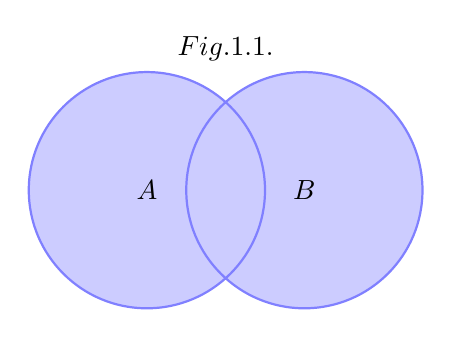
\begin{tikzpicture}
    \draw[filled] \firstcircle node {$A$}
                  \secondcircle node {$B$};
    \node[anchor=south] at (current bounding box.north) {$Fig. 1.1.$};
\end{tikzpicture}
\end{center}
$\square$ Intersection: If there are two sets A and B, then their intersection is
denoted by A $\cap$ B. Let A = $\{2, 3, 4\}$ and B = $\{3, 4, 5, 6\}$. Then, A $\cap$ B =
$\{3, 4\}$. In general, A $\cap$ B = $\{x | x \in A and x \in B\}$.\\
The Venn representation of the intersection operation on two sets can
be represented as shown in Fig. 1.2.\\
\begin{center}
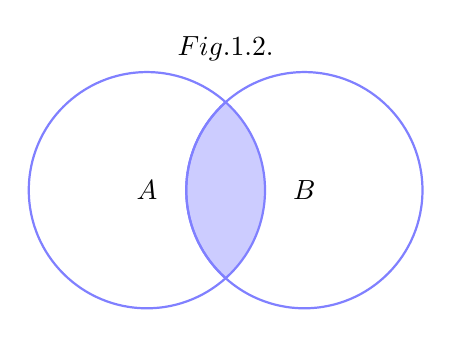
\begin{tikzpicture}
    \begin{scope}
        \clip \firstcircle;
        \fill[filled] \secondcircle;
    \end{scope}
    \draw[outline] \firstcircle node {$A$};
    \draw[outline] \secondcircle node {$B$};
    \node[anchor=south] at (current bounding box.north) {$Fig. 1.2.$};
\end{tikzpicture}
\end{center}
$\square$ Difference: If there are two sets A and B, then their difference is denoted
by $A − B$. Let $A = \{2, 3, 4, 5\}$ and $B = \{3, 4\}$. Then, $A − B = \{2, 5\}$. In
general, $A − B = \{x | x \in A and x \notin  B\}$.\\
The Venn representation of the difference operation on two sets can be
represented as shown in Fig. 1.3.\\
\begin{center}

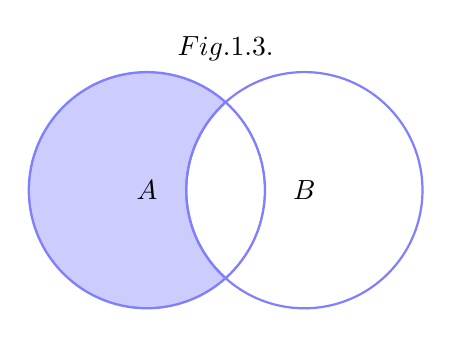
\begin{tikzpicture}
    \begin{scope}
        \clip \firstcircle;
        \draw[filled, even odd rule] \firstcircle node {$A$}
                                     \secondcircle;
    \end{scope}
    \draw[outline] \firstcircle
                   \secondcircle node {$B$};
    \node[anchor=south] at (current bounding box.north) {$Fig. 1.3.$};
\end{tikzpicture}

\end{center}
$\square$ Complementation: The complement of a set A, which is a subset of a
large set U is denoted by AC or $A\prime$ , defi ned by $A\prime = \{x \in U: x \notin  A\}$.\\
The Venn representation of the complement operation is given in
Fig. 1.4.\\
\pgfkeys{not inside/.code={\clip[use path=#1,reverseclip];},
inside/.code={\clip[use path=#1];},
shade/.code=\fill[#1] (current bounding box.south west)rectangle 
(current bounding box.north east);}
\begin{center}
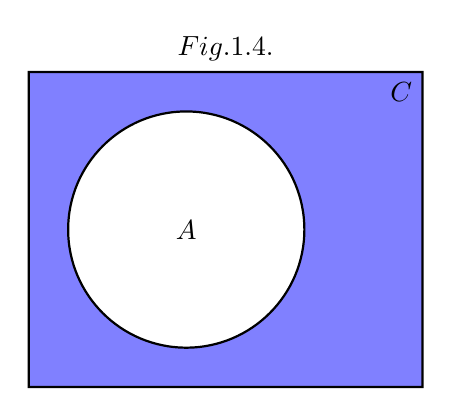
\begin{tikzpicture}
\begin{scope}[yshift=-4.5cm,local bounding box=BL]
   \draw[thick,fill=blue!50,even odd rule] (-0.5,0) node{$A$} circle [radius=1.5cm]
   (-2.5,-2) rectangle (2.5,2) node[below left]{$C$};
   \node[anchor=south] at (current bounding box.north) {$Fig. 1.4.$};
  \end{scope} 
\end{tikzpicture}

\end{center}
$\square$ Cartesian product: If there are two sets A and B, then their Cartesian
product is denoted by $A \times B$. Let $A = \{2, 3, 4, 5\}$ and $B = \{3, 4\}$. Then,
$A \times B = \{(2, 3), (2, 4), (3, 3), (3, 4),(4, 3), (4, 4), (5, 3), (5, 4)\}$. In general,
$A \times B = \{(a, b)|a \in$ A and b $\in B\}$.\\
$\square$ Power set: The power set of a set A is the set of all possible subsets of A.\\
Let $A = \{a, b\}$. Then, the power set of A is $\{(\varnothing), (a), (b), (a, b)\}$. For a set
of elements n, the number of elements of the power set of A is 2n.\\
$\square$ Concatenation: If there are two sets A and B, then their concatenation is
denoted by A.B. Let A = $\{a, b\}$ and B = $\{c, d\}$. Then, A.B = $\{ac, ad, bc,bd\}$. In general, A.B = $\{$ab|a is in A and b is in B$\}$.\\
\textbf{1.2.5 Properties Related to Basic Operation} \\
Some properties related to basic operations on set are as follows:\\
$\square$ A $\cup$ $\varnothing$ = A, A $\cap$ $\varnothing$ = A ($\varnothing$ is called null set)\\
$\square$ A $\cup$ U = U, A $\cap$ U = A (where A $\subset$ U)\\
$\square$ A $\cup$ A = A, A $\cap$ A = A (idempotent law)\\
\end{document}
